\textbf{Ejercicio 1.} Diseñar un circuito lógico que controle el movimiento de un 
ascensor en un edificio de 3 pisos, respondiendo a las solicitudes de usuarios 
según las siguientes especificaciones:

\begin{enumerate}[label=\alph*)]
    \item Botones por piso.
        \begin{itemize}
            \item Piso 1: Botón de subida \textbf{S1}.
            \item Piso 2: Botón de subida \textbf{S2} y de bajada \textbf{B2}.
            \item Piso 3: Botón  de bajada \textbf{B3}.
        \end{itemize}
    \item Debe subir si existe una solicitud de subida y el ascensor está en un piso inferior al solicitado.
    \item Debe bajar si hay una solicitud de bajada y el ascensor está en un piso superior al solicitado.
    \item Debe detenerse al llegar al piso destino.
\end{enumerate}

\textbf{Solución}

Para la implementación de este circuito lógico solo considaremos los casos posibles que se pueden dar. Por 
ejemplo, no se considerará el caso en el que se presione el botón de subida del piso 2 cuando el ascensor 
se encuentra en el piso 3. 

Consideraremos que además de nuestros cuatro botones, tendremos otras tres entradas que nos dirán en qué 
piso se encuentra el ascensor, además, tendremos tres salidas, las cuales indicarán si el ascensor sube, baja o 
está detenido.

Vamos a considerar la siguiente tabla:

\begin{center}
    \begin{tabular}{|c c c c|c c c|c c c|}
        \hline
        $S_1$ & $S_2$ & $B_2$ & $B_3$ & $P_1$ & $P_2$ & $P_3$ & $S$ & $B$ & $P$ \\
        \hline
        \rowcolor{green!30}
        0 & 0 & 0 & 0 & 1 & 0 & 0 & 0 & 0 & 1 \\
        \rowcolor{green!30}
        0 & 0 & 0 & 0 & 0 & 1 & 0 & 0 & 0 & 1 \\
        \rowcolor{green!30}
        0 & 0 & 0 & 0 & 0 & 0 & 1 & 0 & 0 & 1 \\
        \rowcolor{red!30}
        0 & 0 & 0 & 1 & 0 & 0 & 1 & 0 & 1 & 0 \\
        0 & 0 & 0 & 1 & 0 & 1 & 0 & 0 & 0 & 0 \\
        0 & 0 & 0 & 1 & 1 & 0 & 0 & 0 & 0 & 0 \\
        0 & 0 & 1 & 0 & 1 & 0 & 0 & 0 & 0 & 0 \\
        \rowcolor{red!30}
        0 & 0 & 1 & 0 & 0 & 1 & 0 & 0 & 1 & 0 \\
        0 & 0 & 1 & 0 & 0 & 0 & 1 & 0 & 0 & 0 \\
        0 & 1 & 0 & 0 & 0 & 0 & 1 & 0 & 0 & 0 \\
        \rowcolor{blue!30}
        0 & 1 & 0 & 0 & 0 & 1 & 0 & 1 & 0 & 0 \\
        0 & 1 & 0 & 0 & 1 & 0 & 0 & 0 & 0 & 0 \\
        \rowcolor{blue!30}
        1 & 0 & 0 & 0 & 1 & 0 & 0 & 1 & 0 & 0 \\
        1 & 0 & 0 & 0 & 0 & 1 & 0 & 0 & 0 & 0 \\
        1 & 0 & 0 & 0 & 0 & 0 & 1 & 0 & 0 & 0 \\
        \hline
    \end{tabular}
\end{center}

De la cual podemos obtener las expresiones booleanas de las tres salidas, las cuales son:

\begin{align}
\textcolor{green}{P} &= \overline{S_1}\,\overline{S_2}\,\overline{B_2}\,\overline{B_3}\left(P_1\overline{P_2}\,\overline{P_3} + \overline{P_1}P_2\overline{P_3} + \overline{P_1}\,\overline{P_2}P_3\right) \\
\textcolor{blue}{S} &= \overline{B_2}\,\overline{B_3}\,\overline{P_3}\left(\overline{S_1}S_2\overline{P_1}P_2 + S_1\overline{S_2}P_1\overline{P_2}\right) \\
\textcolor{red}{B} &= \overline{S_1}\,\overline{S_2}\,\overline{P_1}\left(\overline{B_2}B_3\overline{P_2}P_3 + B_2\overline{B_3}P_2\overline{P_3}\right)
\end{align}

Ya con las expresiones booleanas podemos implementar el circuito lógico en Logisim. 

\begin{figure}[H]
    \centering
    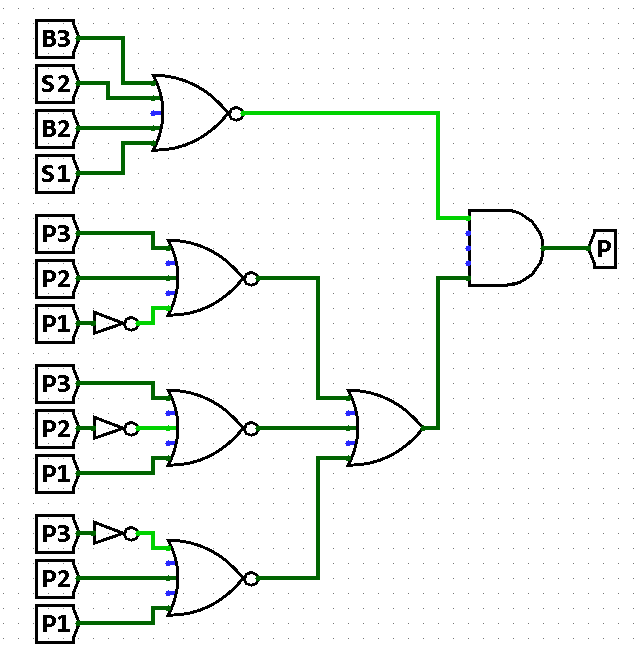
\includegraphics[width=0.8\textwidth]{Salida P.png}
    \caption{Circuito para la salida P (Parada)}
\end{figure}

\begin{figure}[H]
    \centering
    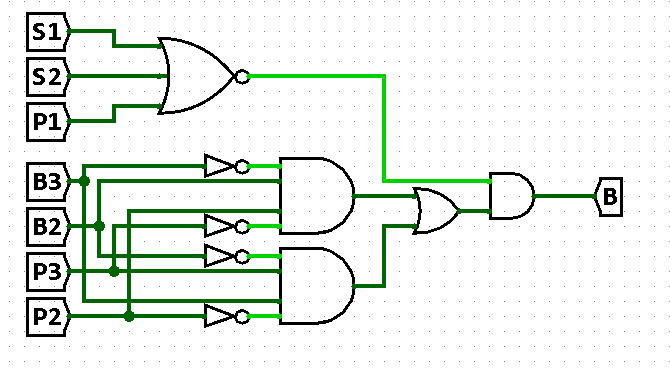
\includegraphics[width=0.8\textwidth]{Salida B.png}
    \caption{Circuito para la salida B (Bajada)}
\end{figure}

\begin{figure}[H]
    \centering
    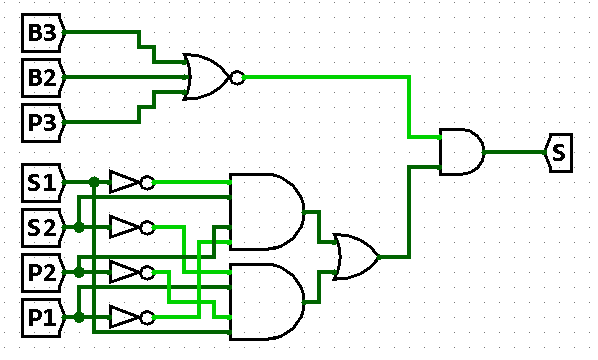
\includegraphics[width=0.8\textwidth]{Salida S.png}
    \caption{Circuito para la salida S (Subida)}

\end{figure}

\begin{figure}[H]
    \centering
    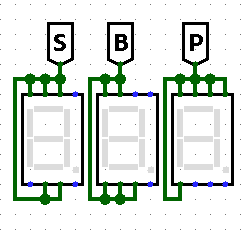
\includegraphics[width=0.8\textwidth]{Salidas.png}
    \caption{Circuito completo con todas las salidas}
\end{figure}

El circuito se hizo de forma modular, para que sea más fácil visualizar los elementos y las conexiones del mismo.


\newpage